%%%%%%%%%%%%%%%%%%%%%%%%%%%%%%%%%%%%%%%%%
% Beamer Presentation
% LaTeX Template
% Version 1.0 (10/11/12)
%
% This template has been downloaded from:
% http://www.LaTeXTemplates.com
%
% License:
% CC BY-NC-SA 3.0 (http://creativecommons.org/licenses/by-nc-sa/3.0/)
%
%%%%%%%%%%%%%%%%%%%%%%%%%%%%%%%%%%%%%%%%%

%----------------------------------------------------------------------------------------
%	PACKAGES AND THEMES
%----------------------------------------------------------------------------------------

\documentclass{beamer}

\usepackage{hyperref}

\mode<presentation> {

% The Beamer class comes with a number of default slide themes
% which change the colors and layouts of slides. Below this is a list
% of all the themes, uncomment each in turn to see what they look like.

%\usetheme{default}
%\usetheme{AnnArbor}
%\usetheme{Antibes}
%\usetheme{Bergen}
%\usetheme{Berkeley}
%\usetheme{Berlin}
%\usetheme{Boadilla}
%\usetheme{CambridgeUS}
%\usetheme{Copenhagen}
%\usetheme{Darmstadt}
%\usetheme{Dresden}
%\usetheme{Frankfurt}
%\usetheme{Goettingen}
%\usetheme{Hannover}
%\usetheme{Ilmenau}
%\usetheme{JuanLesPins}
%\usetheme{Luebeck}
%\usetheme{Madrid}
%\usetheme{Malmoe}
%\usetheme{Marburg}
%\usetheme{Montpellier}
\usetheme{PaloAlto}
%\usetheme{Pittsburgh}
%\usetheme{Rochester}
%\usetheme{Singapore}
%\usetheme{Szeged}
%\usetheme{Warsaw}

% As well as themes, the Beamer class has a number of color themes
% for any slide theme. Uncomment each of these in turn to see how it
% changes the colors of your current slide theme.

%\usecolortheme{albatross}
%\usecolortheme{beaver}
%\usecolortheme{beetle}
%\usecolortheme{crane}
%\usecolortheme{dolphin}
%\usecolortheme{dove}
%\usecolortheme{fly}
%\usecolortheme{lily}
%\usecolortheme{orchid}
%\usecolortheme{rose}
%\usecolortheme{seagull}
\usecolortheme{seahorse}
%\usecolortheme{whale}
%\usecolortheme{wolverine}

%\setbeamertemplate{footline} % To remove the footer line in all slides uncomment this line
%\setbeamertemplate{footline}[page number] % To replace the footer line in all slides with a simple slide count uncomment this line

%\setbeamertemplate{navigation symbols}{} % To remove the navigation symbols from the bottom of all slides uncomment this line
}

\usepackage{graphicx} % Allows including images
\usepackage{booktabs} % Allows the use of \toprule, \midrule and \bottomrule in tables
\usepackage{scrextend}

%----------------------------------------------------------------------------------------
%	TITLE PAGE
%----------------------------------------------------------------------------------------

\title[Meta-Heuristics]{Meta-Heuristics} % The short title appears at the bottom of every slide, the full title is only on the title page

\author{Collin Price \& Ron Bond} % Your name
\institute[Brock University] % Your institution as it will appear on the bottom of every slide, may be shorthand to save space
{
%Brock University \\ % Your institution for the title page
\medskip
%\textit{john@smith.com} % Your email address
}
\date{May 12, 2014} % Date, can be changed to a custom date

\begin{document}

\begin{frame}
\titlepage % Print the title page as the first slide
\end{frame}

\begin{frame}
\frametitle{Overview} % Table of contents slide, comment this block out to remove it
\tableofcontents % Throughout your presentation, if you choose to use \section{} and \subsection{} commands, these will automatically be printed on this slide as an overview of your presentation
\end{frame}

%----------------------------------------------------------------------------------------
%	PRESENTATION SLIDES
%----------------------------------------------------------------------------------------

%------------------------------------------------
\section{Optimization}
%------------------------------------------------
% optimization
\begin{frame}
\frametitle{Optimization}
\begin{columns}[c]
\column{.70\textwidth}
\textbf{Objective}
\begin{itemize}
\item Minimize/maximize an objective output whose value(s) depend on a set of input variables
\item Function often referred to as "Fitness Function"
\end{itemize}

\textbf{Landscape}
\begin{itemize}
\item The n-dimensional mapping of input to output values:
\item inputs are parameters to be optimized
\item outputs are the "fitness" or score of the given input configuration
\end{itemize}

\column{.20\textwidth}
\begin{figure}
\centering
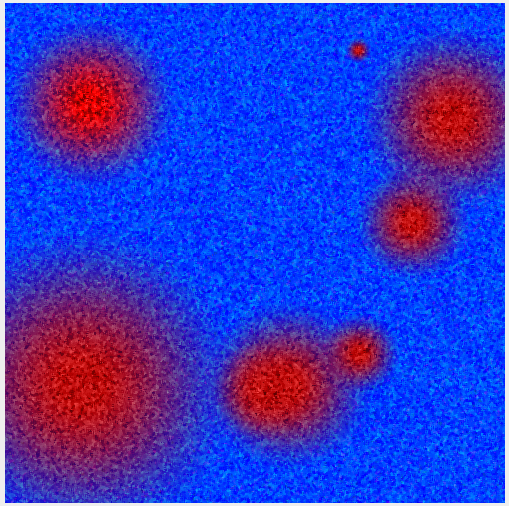
\includegraphics[width=20mm]{func.png}
\caption{Fitness Landscape}
\label{exampleFunction}
\end{figure}

\end{columns}
\end{frame}

%------------------------------------------------
\section{Metaheuristics}
%------------------------------------------------
\subsection{Metaheuristics? Why?}
% meta def
\begin{frame}
\frametitle{Metaheuristics}
\textbf{Metaheuristics}
\begin{itemize}
\item Partial search algorithm
\item Often stochastic in nature
\item Do not guarantee a globally optimal solution
\end{itemize}

\textbf{Why Metaheuristics?}
\begin{itemize}
\item Incomplete or imperfect information
\item Limited computation capacity
\end{itemize}

\end{frame}

%------------------------------------------------
\subsection{Classifications}
% meta-classes
\begin{frame}
\frametitle{Classifications}
\begin{figure}
\centering
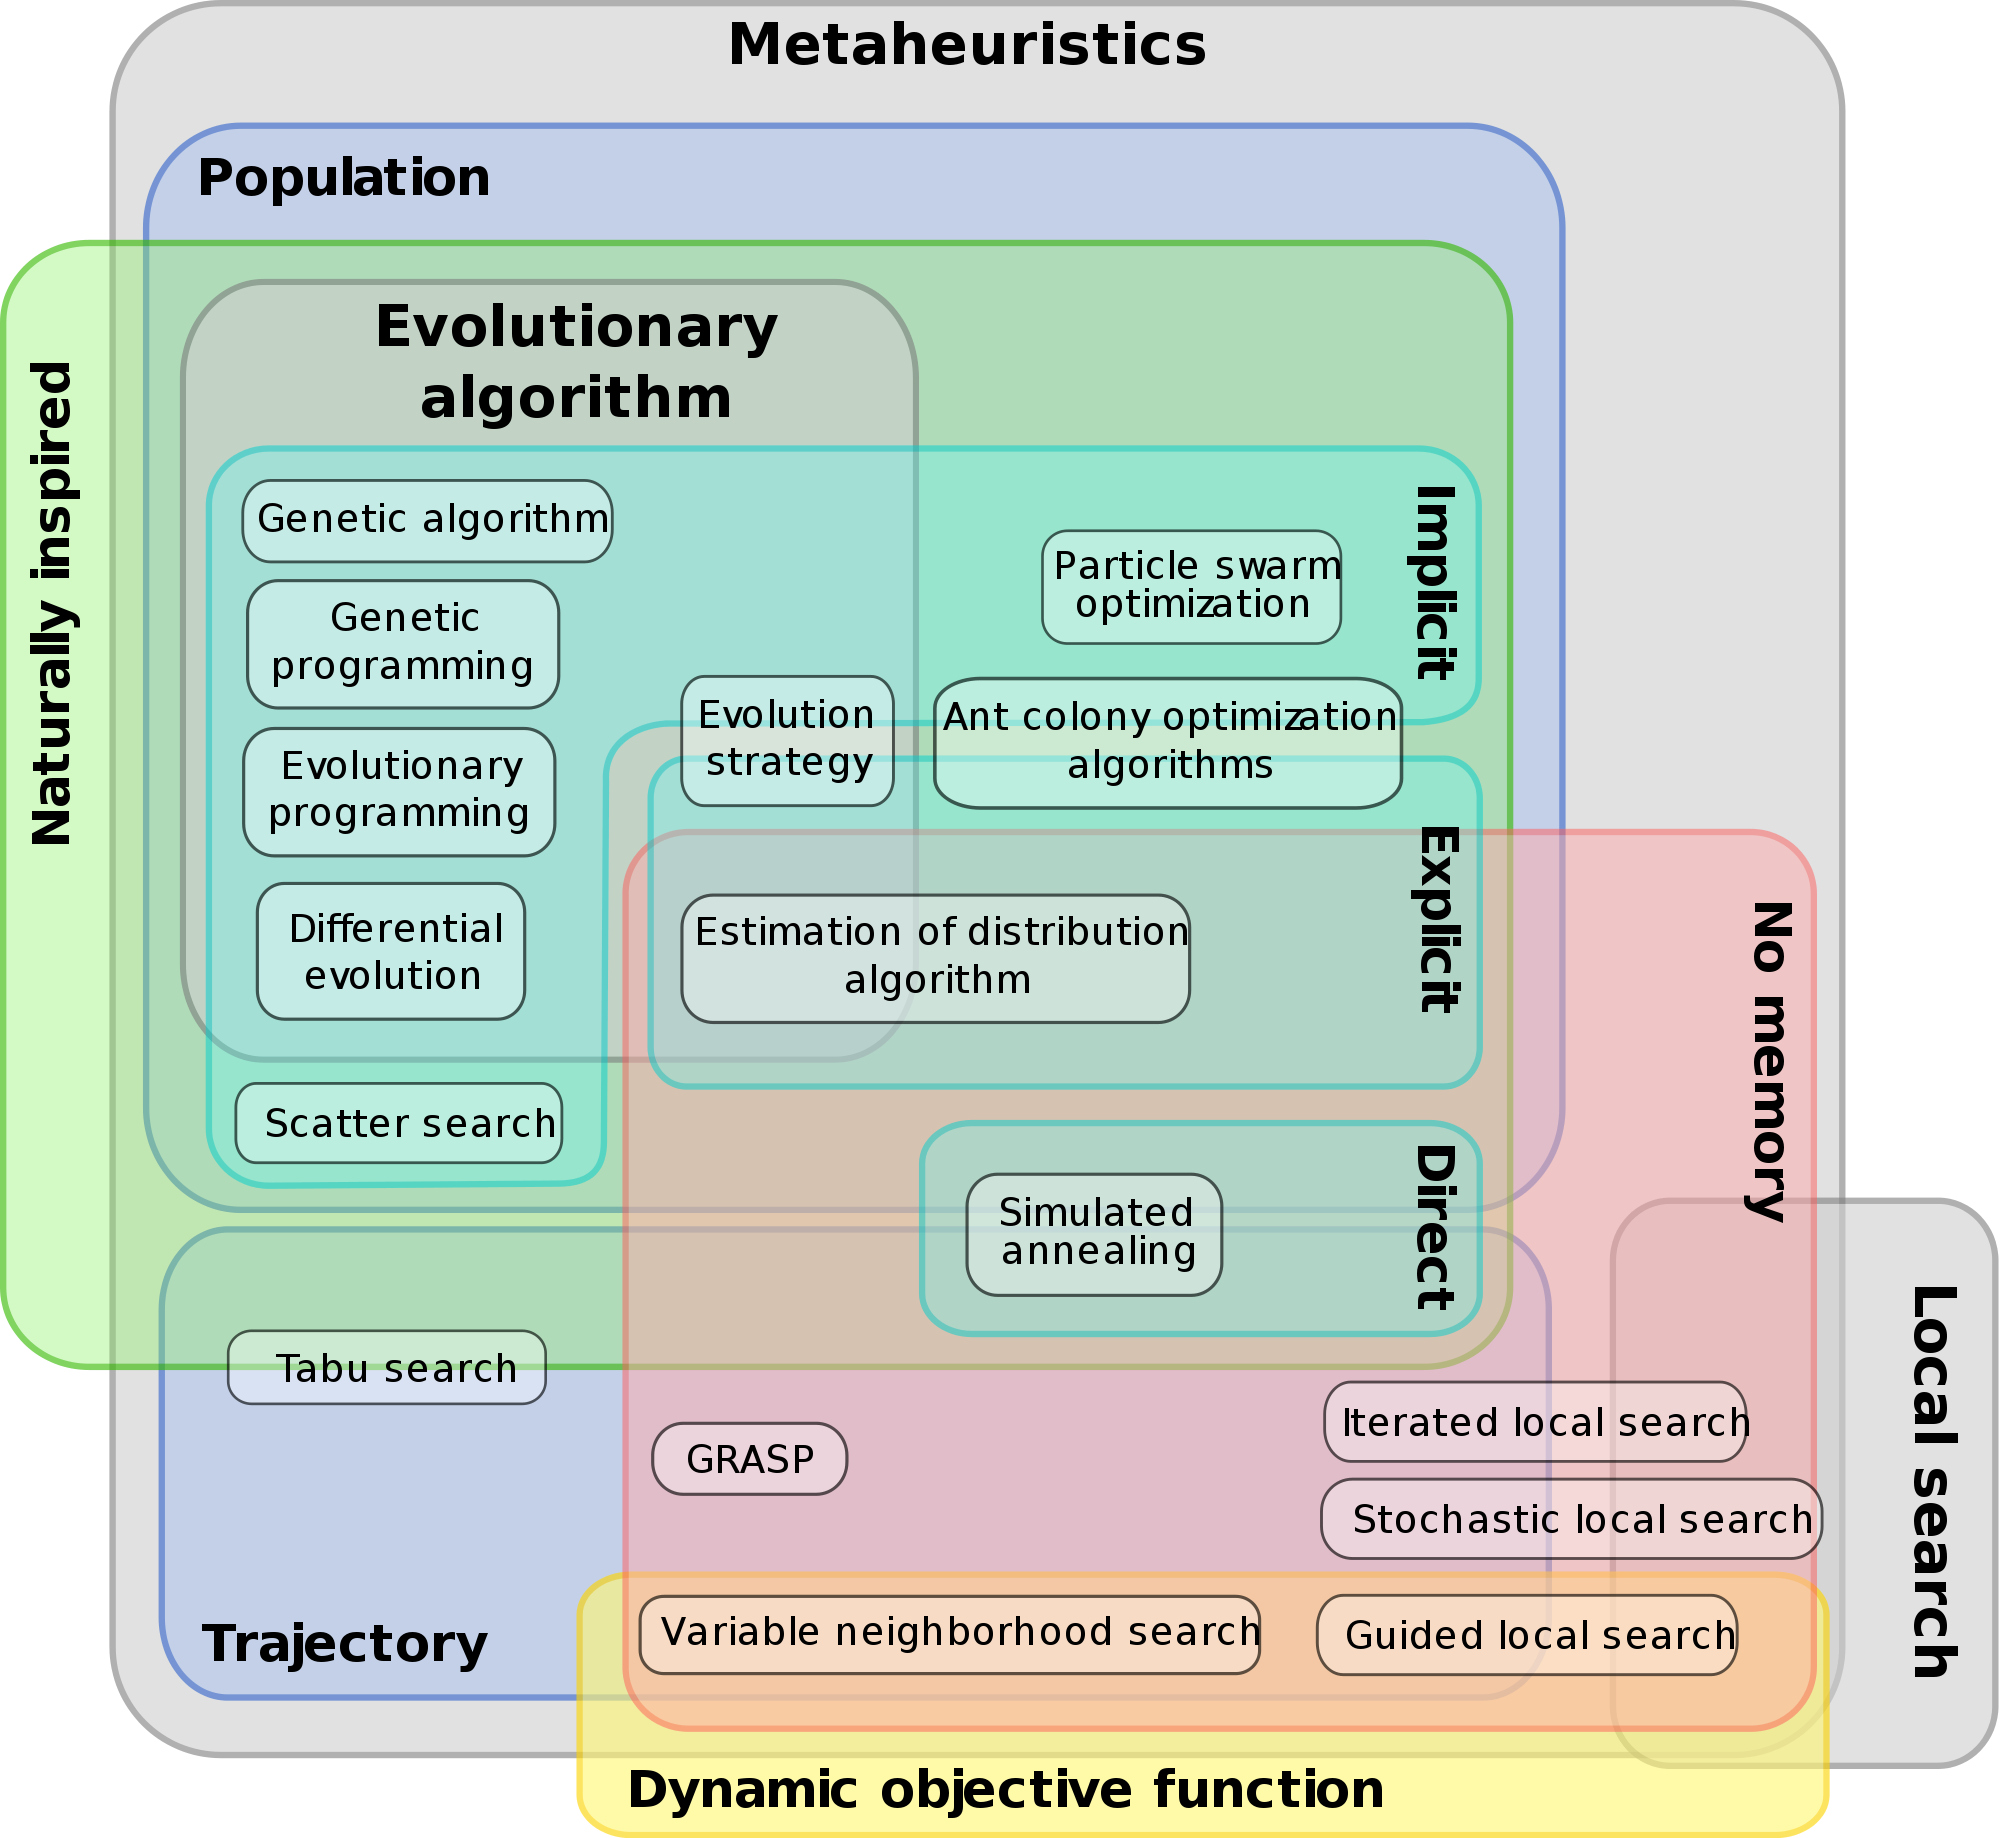
\includegraphics[width=70mm ]{metaClasses.png}
\caption{Metaheuristic Clasifications}
\label{classes}
\end{figure}
\end{frame}

%------------------------------------------------
\section{Metaheuristic Examples}
%------------------------------------------------
\subsection{Genetic Algorithms}

\begin{frame}

	\frametitle{Iterative Framework Overview}

	\begin{figure}
		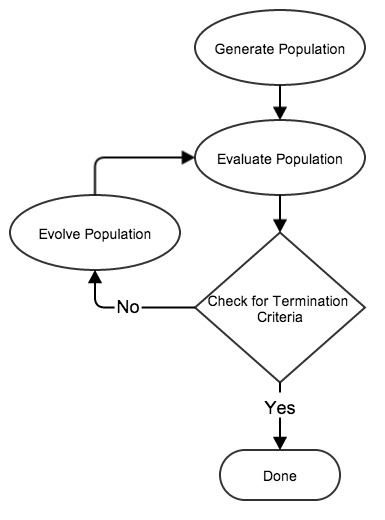
\includegraphics[width=50mm]{resources/general_flowchart.jpg}
	\end{figure}

\end{frame}

\begin{frame}

	\frametitle{Genetic Algorithm}

	\begin{itemize}
		\item A search heuristic that mimics the process of natural selection.
		\item Individuals are combined and modified to create new ones.
	\end{itemize}

\end{frame}

\begin{frame}

	\frametitle{Individuals}

	\begin{itemize}
		\item Represents a proposed solution to the problem.
		\item Commonly represented as an array.
		\item Representations can vary depending on the problem.
	\end{itemize}

	\begin{figure}
		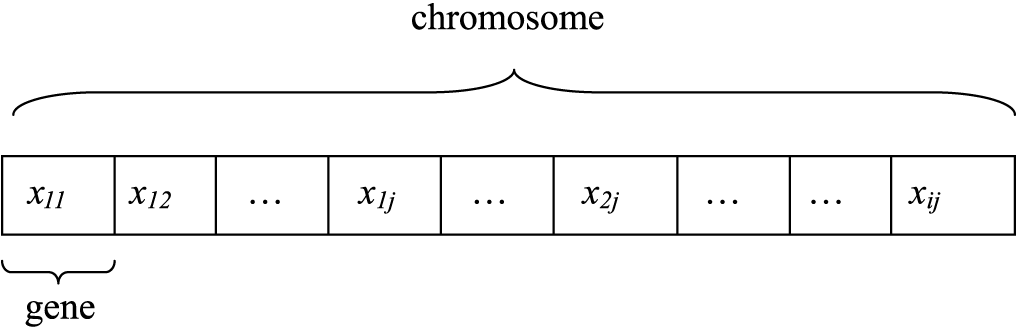
\includegraphics[width=90mm]{resources/chromosome.png}
	\end{figure}

\end{frame}

\begin{frame}

	\frametitle{Crossover}

	\begin{figure}
		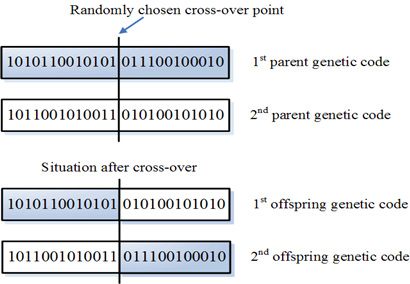
\includegraphics[width=80mm]{resources/crossover.png}
	\end{figure}

\end{frame}

\begin{frame}

	\frametitle{Mutation}

	\begin{figure}
		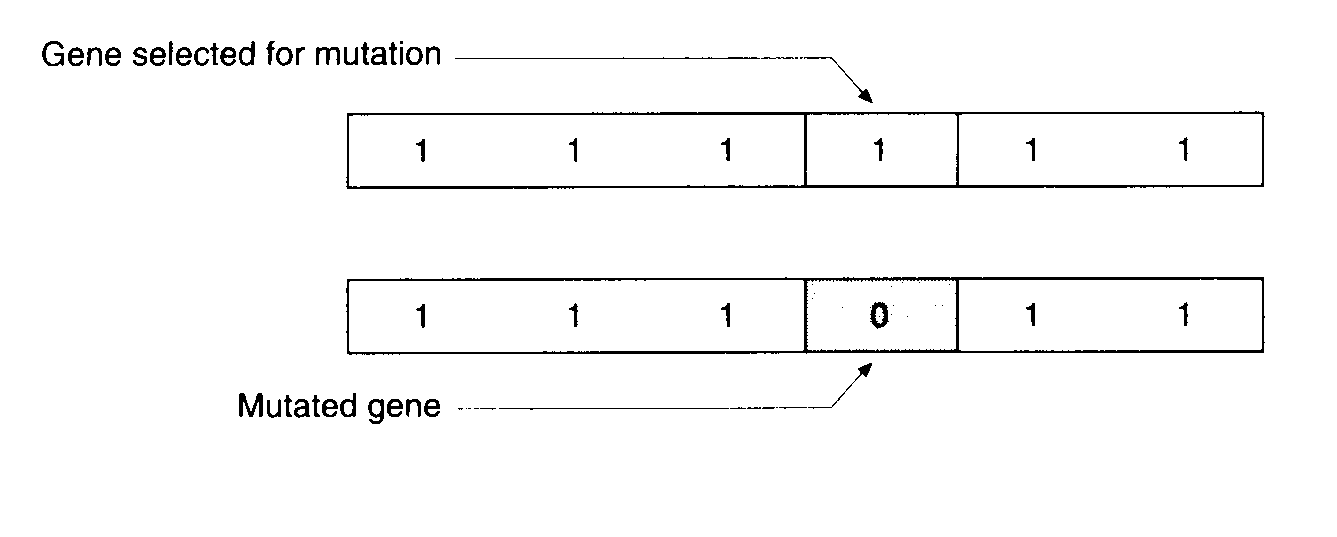
\includegraphics[width=100mm]{resources/mutation2.png}
	\end{figure}

\end{frame}

\begin{frame}

	\frametitle{Selection}

	\begin{itemize}
		\item Method used to select individuals from the population for breeding.
		\item Example: Tournament Selection
		\begin{itemize}
			\item Randomly choose n-individuals from the population.
			\item Select the individual with the best fitness.
		\end{itemize}
	\end{itemize}

\end{frame}

\begin{frame}

	\frametitle{Parameters}

	\begin{itemize}
		\item There are several parameters that can be tuned to change the results of your genetic algorithm.
		\item There is no optimal set of parameters. Parameter values are empirically found.
		\item Parameters:
			\begin{itemize}
				\item Number of Generations
				\item Population Size
				\item Crossover Rate
				\item Mutation Rate
				\item Elitism?
			\end{itemize}
	\end{itemize}

\end{frame}

%------------------------------------------------
\subsection{Particle Swarm Optimization}
% PSO
\begin{frame}
\frametitle{Particle Swarm Optimization}

\begin{columns}[c]

\column{.33\textwidth}

\begin{figure}
\centering
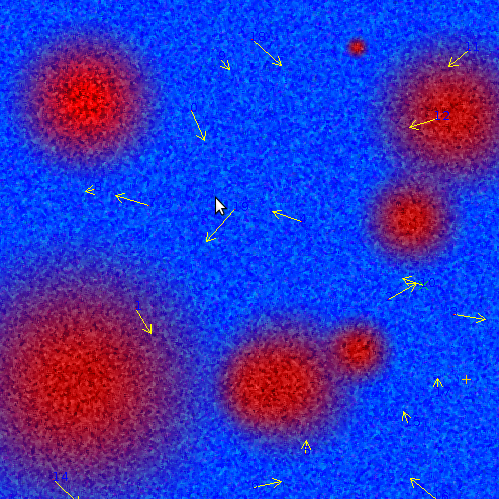
\includegraphics[width=35mm ]{funcStart.png}
\end{figure}

\column{.33\textwidth}
\begin{figure}
\centering
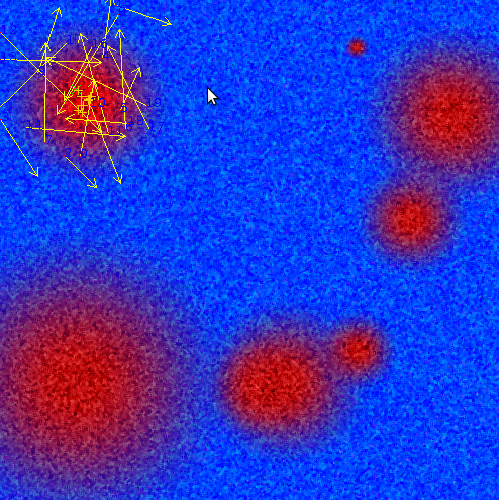
\includegraphics[width=35mm ]{funcFound.png}
\end{figure}

\column{.33\textwidth}
\begin{figure}
\centering
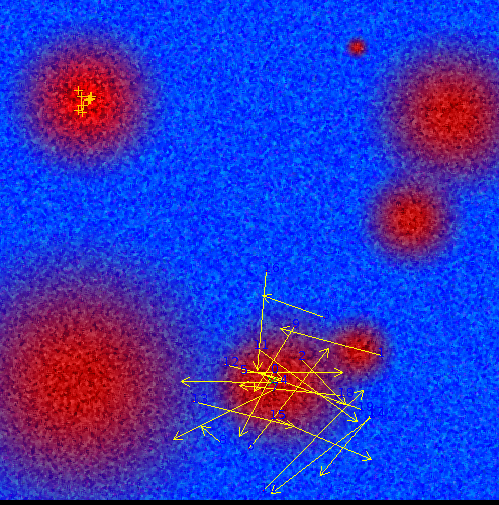
\includegraphics[width=35mm]{funcNotFound.png}
\end{figure}
\end{columns}

\begin{figure}
\centering
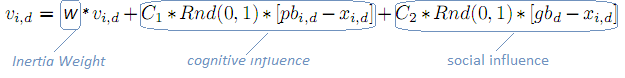
\includegraphics[width=70mm ]{psoEq.png}
\caption{Original PSO Behaviour}
\label{pso}
\end{figure}

\end{frame}

%------------------------------------------------
\subsection{Genetic Programming}

\begin{frame}

	\frametitle{Genetic Programming}

	\begin{itemize}
		\item Specialization of a genetic algorithm.
		\item Each individual is a computer program.
		\item Traditionally represented as tree structures.
	\end{itemize}

\end{frame}

\begin{frame}

	\frametitle{Individuals}

	\begin{itemize}
		\item Individuals randomly generated from a list of operators and terminals.
		\item Example Operators: addition, subtraction, multiplication, cosine.
		\item Example Terminals: ephemeral random constants, problem specific numbers.
	\end{itemize}

\end{frame}

\begin{frame}
	\frametitle{Crossover \& Mutation}
	\begin{figure}
		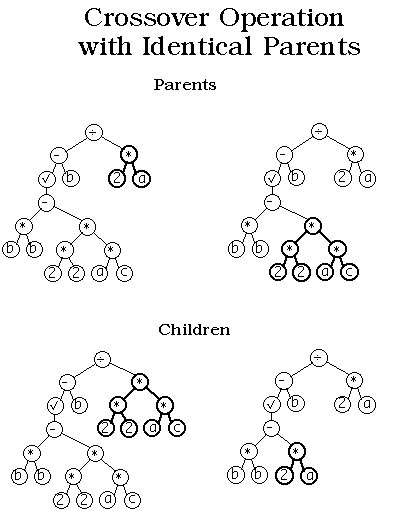
\includegraphics[width=50mm ]{resources/gp-crossover.png}
	\end{figure}

\end{frame}

%------------------------------------------------
\subsection{Solution \& Fitness Representation}

\begin{frame}
\frametitle{Solution \& Fitness Representation}
	
	\begin{itemize}
		\item Performance of Metaheuristics are limited to the information given
		\item "information" is encoded in
		\begin{itemize}
			\item Solution Representation
			\item Fitness Function
		\end{itemize}
	\end{itemize}

	\begin{columns}[c]
	\column{.50\textwidth}
	\begin{figure}
	\centering
		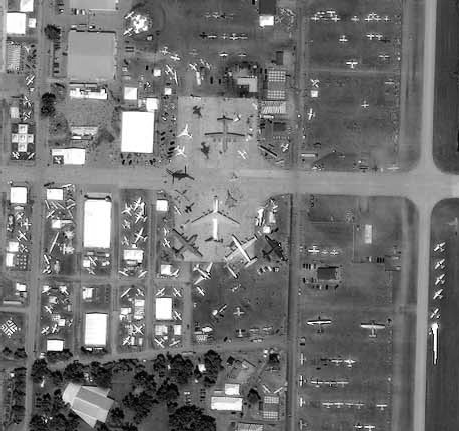
\includegraphics[width=35mm ]{resources/airplane-original-min.png}
	\end{figure}

	\column{.50\textwidth}
	\begin{figure}
	\centering
		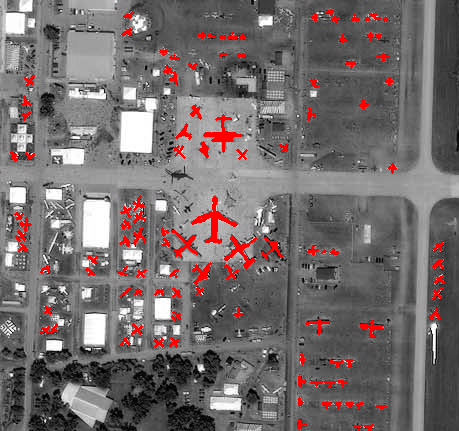
\includegraphics[width=35mm ]{resources/airplane-ground-truth-min.png}
	\end{figure}
	\end{columns}

\end{frame}

\begin{frame}
\frametitle{Representation - Efficiency}
	
	\begin{itemize}
		\item Search space grows with the size of the language
		\item Minimizing the language reduces search complexity
		\item Example: Language 1 (left) vs Language 2 (right)
	\end{itemize}
	
\begin{columns}[c]
\column{.40\textwidth}
\begin{figure}
\begin{itemize}
		\item add(x,y)
		\item sub(x,y)
		\item mult(x,y)
		\item div(x,y)
		\item log(x)
		\item max(x,y)
\end{itemize}
\end{figure}

\column{.40\textwidth}
\begin{figure}
\begin{itemize}
		\item sub(x,y)
		\item mult(x,y)
		\item max(x,y)
\end{itemize}
\end{figure}
\end{columns}	

\end{frame}


\begin{frame}
\frametitle{Representation - Language}
	
	\begin{itemize}
		\item Language components offer different information
		\item Derivative components can offer "new information" and reduce search space
		\item Example: Simple (left) vs Derived (right)
	\end{itemize}
	
\begin{columns}[c]
\column{.40\textwidth}
\begin{figure}
\begin{itemize}
		\item sub(x,y)
		\item mult(x,y)
		\item max(x,y)
\end{itemize}
\end{figure}

\column{.40\textwidth}
\begin{figure}
\begin{itemize}
		\item Edge Filters
		\item Geometric Filter
		\item ...
		
\end{itemize}
\end{figure}
\end{columns}	

\end{frame}


\begin{frame}
\frametitle{Representation}

\begin{columns}[c]

\column{.50\textwidth}
\begin{figure}
\centering
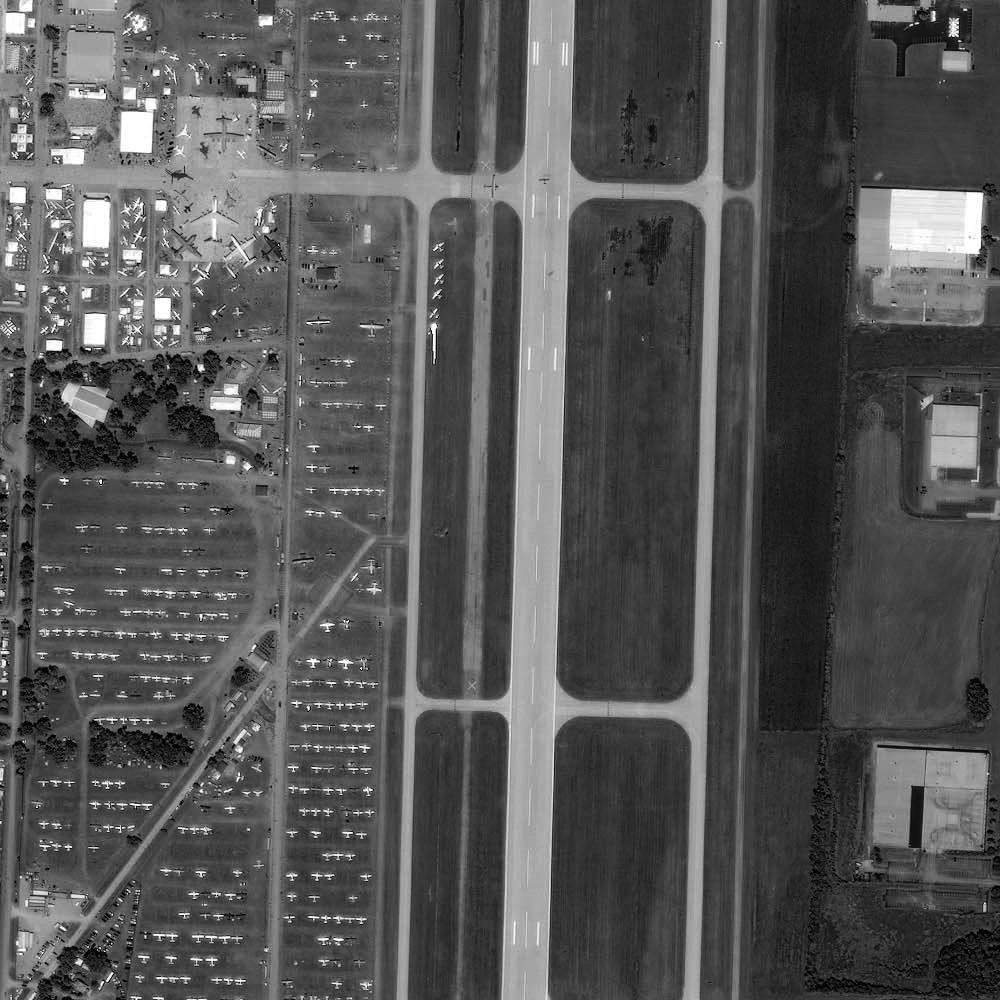
\includegraphics[width=50mm ]{resources/airplane-original.jpg}
\end{figure}

\column{.50\textwidth}
\begin{figure}
\centering
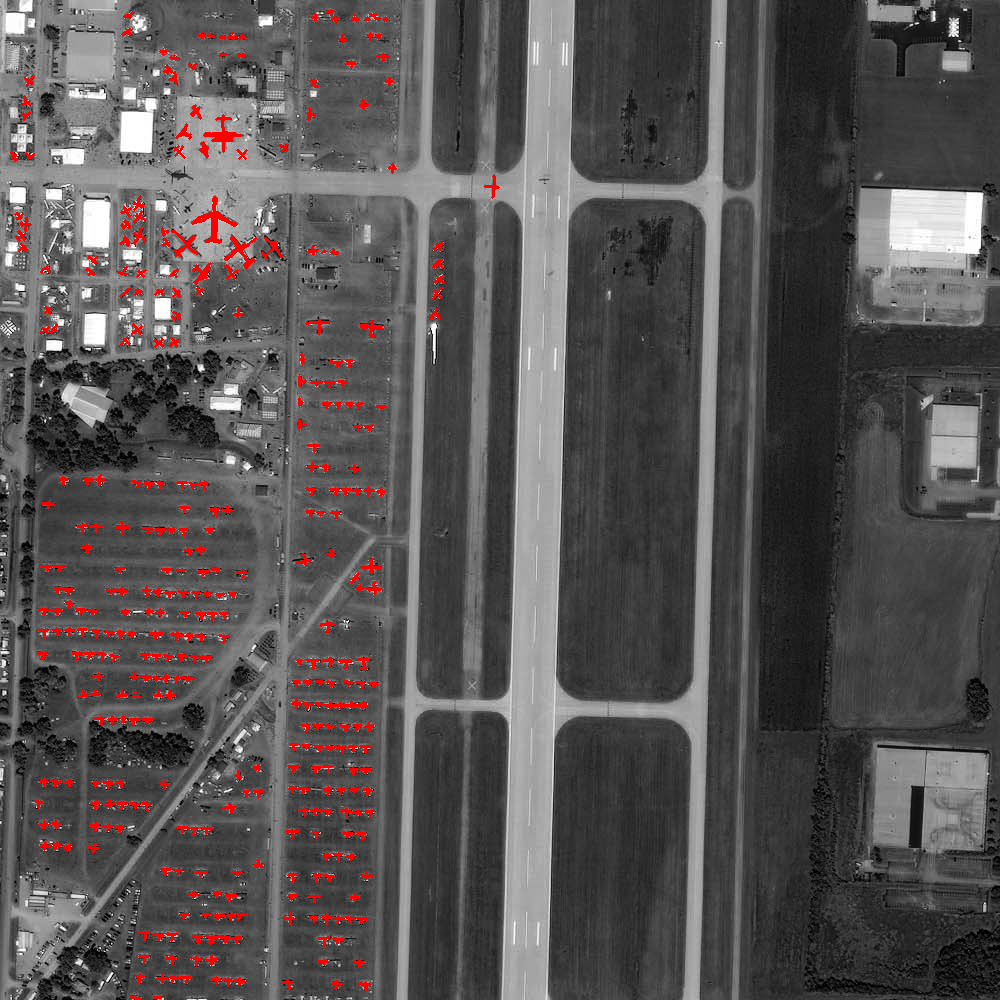
\includegraphics[width=50mm ]{resources/airplane-ground-truth.jpg}
\end{figure}
\end{columns}

\end{frame}

%------------------------------------------------
\begin{frame}
\frametitle{Fitness Function}

	\begin{itemize}
		\item Produces values on which to compare generated solutions
		\item Defines the "desired solution"
		\item Fitness function will therefore impact performance
	\end{itemize}
	
	\begin{columns}[c]
	\column{.50\textwidth}
	\begin{figure}
	\centering
		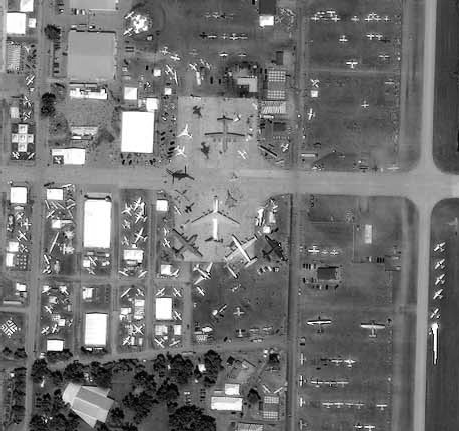
\includegraphics[width=30mm ]{resources/airplane-original-min.png}
		\caption{f(x) = Max(true positives)}
	\end{figure}

	\column{.50\textwidth}
	\begin{figure}
	\centering
		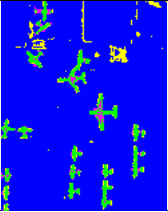
\includegraphics[width=30mm ]{resources/airplane-result.png}
		\caption{f(x) = Min(false positives + false negatives)}
	\end{figure}
	\end{columns}

\end{frame}

%------------------------------------------------
\section{Applications}
%------------------------------------------------
\begin{frame}
\frametitle{Applications}

\begin{itemize}
	\item \href{http://nn.cs.utexas.edu/nero/gallery.php}{NERO - Evolved Neural Networks}
	\item \href{http://www.rockpapershotgun.com/2010/11/02/genetic-algorithms-find-build-order-from-hell}{Starcraft 2 build orders - Genetic Algorithm}
	\item \href{http://en.wikipedia.org/wiki/Evolved_antenna}{Evolved Antenna - Evolutionary Algorithm}
	\item \href{http://boxcar2d.com/index.html}{Boxcar 2D - Genetic Algorithm}
	\item \href{https://www.youtube.com/watch?v=bBt0imn77Zg}{Evolving Virtual Creatures}
\end{itemize}

\end{frame}

%------------------------------------------------
\section{Metaheuristic limitations}
%------------------------------------------------

\subsection{No Free Lunch}
% No free lunch theorem
\begin{frame}
\frametitle{No Free Lunch theorem}
\begin{block}{No Free Lunch - Wolpert/Macready 1997}
For all possible performance measures, no search algorithm is better than another when its performance is averaged over all possible discrete functions.
\end{block}

\textbf{}
\begin{itemize}
\item No silver bullet
\item Does not state that algorithms cannot generalize to categories of problems
\end{itemize}

\end{frame}
%------------------------------------------------
\subsection{Optimizing Optimizers}
% recursive optimization
\begin{frame}
\frametitle{Optimizing Optimizers}

\textbf{Optimizing Optimizers}
\begin{itemize}
\item Metaheuristics are general because they can be tuned to a specific problem
\item Tuning is itself an optimization problem
\item Trading one search space for another
\end{itemize}

\textbf{Apply Another Metaheuristic}
\begin{itemize}
\item Same problem exists for the higher-level heuristic
\item computation increases exponentially

\end{itemize}

\end{frame}


%------------------------------------------------

\begin{frame}
\Huge{\centerline{Questions?}}
\end{frame}

%----------------------------------------------------------------------------------------

\end{document} 